\newpage
\section{Matrix Multiplication}
\subsection{GPU: naive}
\begin{figure}[h]
    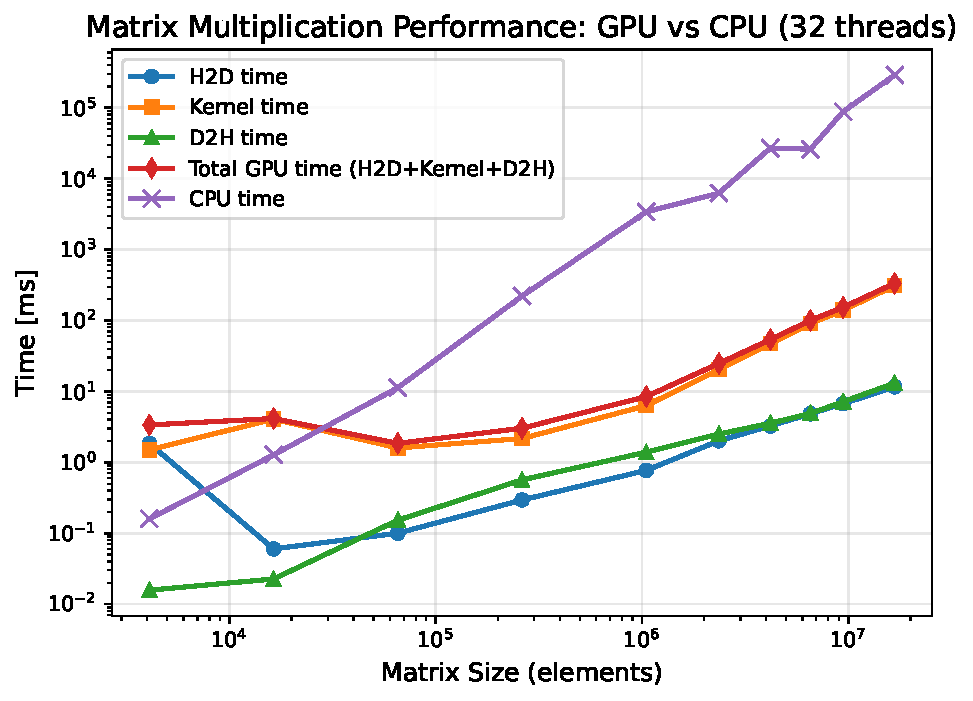
\includegraphics[scale=0.7]{../plots_miro/performance.pdf}
    \caption{Performance comparison 32 threads/block}
    \label{fig:5.2a}
\end{figure}
\ref{fig:5.2a} shows the performance of the multiplication and the data movements for different matrix sizes. While the transfer times increase with larger matrices, they are always dominated by the computation time being approx. one order of magnitude larger.\\
Compared to the version on the CPU, the comparison shows that the speedup sharply increases with matrix size until approx. 1 Million elements.\\
The maximum speedup measured is for a matrix size of 4096x4096 with a speedup of 934 for just the calculation and a speedup of 865 when including the time for the data movement.\\
\begin{figure}[h]
    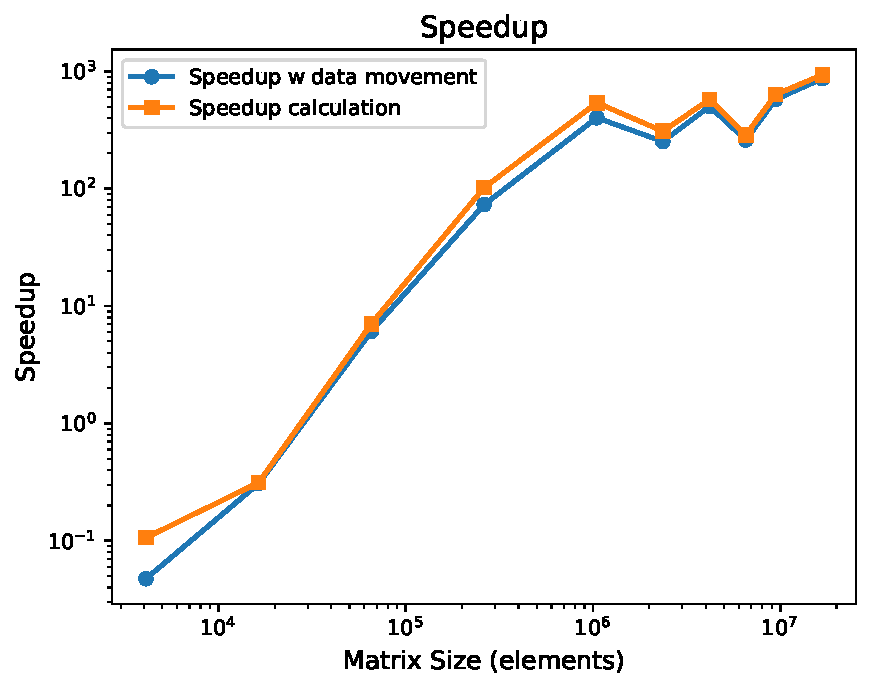
\includegraphics[scale=0.7]{../plots_miro/speedup.pdf}
    \caption{Speedup 32 threads/block}
    \label{fig:5.2b}
\end{figure}
\FloatBarrier
With regards to scaling the threads per block, we can see in \ref{fig:5.2c} and \ref{fig:5.2d} that (excluding some outliers) the runtime decreases especially for the initial increase from 1 to 8 threads per block. After that the improvements are smaller, with thread sizes which are not a power of 2 performing worse than their surrounding powers of 2.\\
\begin{figure}[h]
    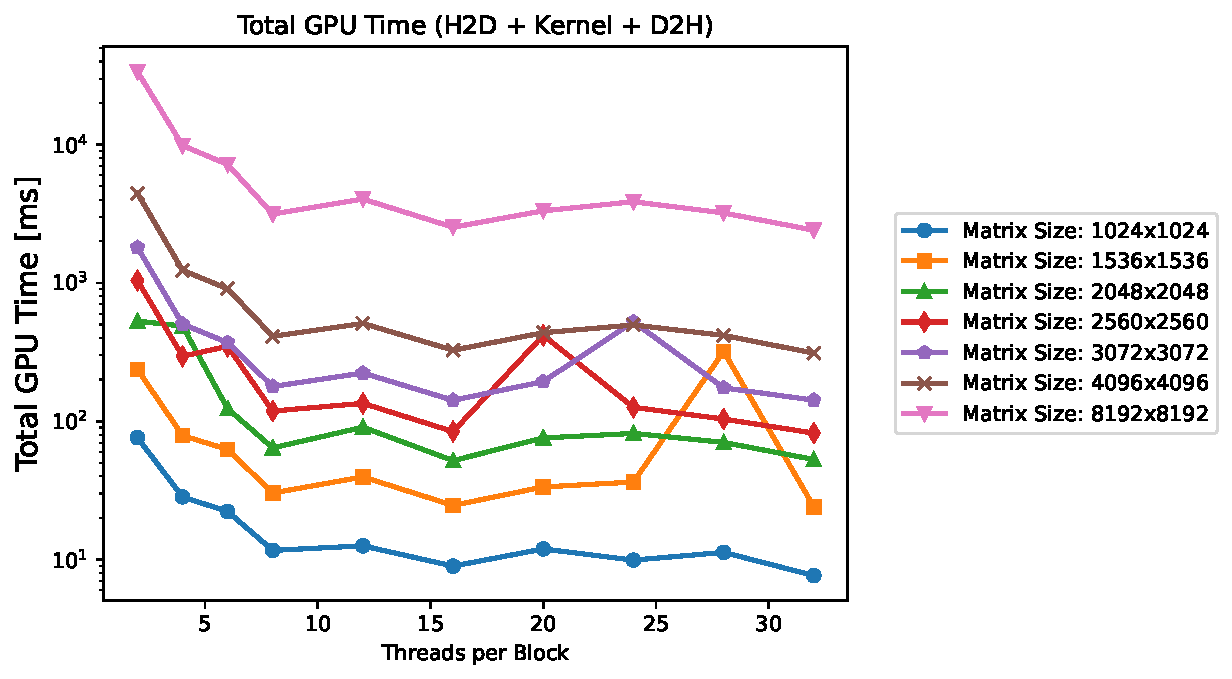
\includegraphics[scale=0.7]{../plots_miro/threads.pdf}
    \caption{Speedup 32 threads/block}
    \label{fig:5.2c}
\end{figure}
\\
\begin{figure}
    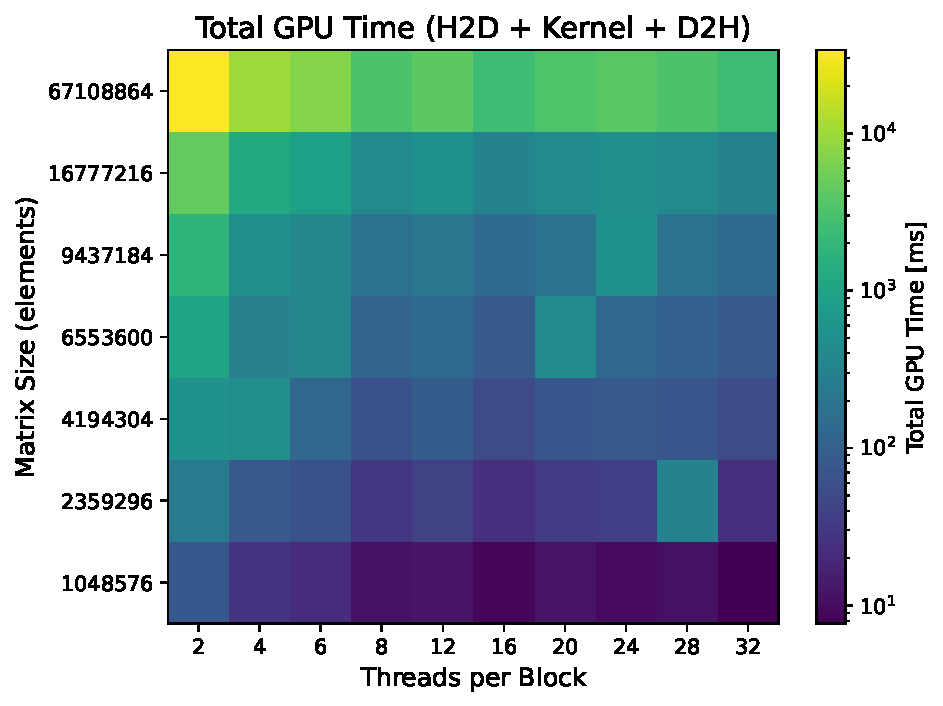
\includegraphics[scale=0.7]{../plots_miro/threads_heatmap.pdf}
    \caption{Speedup 32 threads/block}
    \label{fig:5.2d}
\end{figure}
\FloatBarrier